\documentclass[DeGregorioResumen]{subfiles}
\setcounter{section}{2}
\begin{document}
\part*{Macroeconomía I}
\section{Consumo}
\subsection{La función de consumo keynesiana}
Esta teoría plantea que el principal determinante del consumo en el período $t$ es el ingreso disponible durante dicho período:
\begin{equation}
C_t=\overline{C}+c\underbrace{(Y_t-T_t)}_{Y^d_t}.
\label{eq:consumo_keynesiano}
\end{equation}
\begin{where}
\item[C] es consumo y $\overline{C}$ es consumo autónomo, correspondiente a un consumo ``basal'' de cada período, el cual es independiente de las condiciones económicas o de los ingresos.
\item[Y^d] es el ingreso disponible después de pagar impuestos.
\item[c] es la propensión marginal a consumir ($PMgC $) con respecto del ingreso disponible.
\begin{equation*}
c=PMgC=\frac{\partial C}{ \partial (Y-T)} < 1,
\end{equation*} 
donde $c \in [0,1]$ y puede interpretarse como el complemento de la propensión marginal al ahorro: $s=1-c$.
\end{where}

El consumo keynesiano expresado en \eqref{eq:consumo_keynesiano} se grafica en la \autoref{fig03_01-consumo_keynesiano}. La propensión media a consumir se obtiene al dividir dicha ecuación de consumo por $Y^d$,
\begin{equation*}
PMeC=\frac{C}{Y-T}=c+\frac{\overline{C}}{Y-T}.
\end{equation*}

\begin{figure}[h]
\centering
\def\svgwidth{0.5\textwidth}
\import{monos/}{fig03_01-consumo_keynesiano.pdf_tex}
\caption{Función de consumo keynesiana}
\label{fig03_01-consumo_keynesiano}
\end{figure}

Si bien la función de consumo keynesiana es útil para períodos relativamente largos, presenta problemas de predicción para períodos breves ya que es incapaz de lidiar adecuadamente con cambios bruscos del consumo. Además, esta teoría predice que la $PMeC$ tendría un movimiento secular a la baja (convergiendo en $c$), cosa que no pareciera ocurrir en realidad.

\subsection{Restricción presupuestaria intertemporal}

Se consideran ahora teorías de consumo intertemporales que permiten ahorro y deuda. Primero se examinan los ingresos, los que se definen como
\begin{equation}
Y_t=Y_{l,t}+r\cdot A_t,
\end{equation}
donde $Y_{l,t}$ son los ingresos del trabajo y $A_t$ son activos netos. La acumulación de activos es ahorro y ocurre cuando $A_{t+1}>A_t$.

Se hace el supuesto que el ingreso total debe ser igual al gasto total, es decir, $Y_{l,t}+rA_t=C_t+T_t+A_{t+1}-A_t$. Esto puede reescribirse como
\begin{equation*}
A_{t+1}=Y_{l,t}+A_t(1+r)-C_t-T_t \quad \forall \; t.
\end{equation*}

Esta ecuación puede resolverse recursivamente para $N$ períodos, asumiendo que $A_t$ contiene toda la información relevante para períodos anteriores a $t$. Por lo tanto, se puede encontrar $A_{t+2}$ reemplazando el valor de $A_{t+1}$ y así sucesivamente, hasta llegar a
\begin{equation*}
(1+r)A_t=\sum_{s=0}^N\frac{C_{t+s}+T_{t+s}-Y_{l,t+s}}{(1+r)^s}+\cancelto{0}{\frac{A_{t+N+1}}{(1+r)^N}}.
\end{equation*}

Notar que el último término se cancela porque se supone que no se dejan activos acumulados para un período superior a $N$, es decir, se supone que que no hay herencias. Despejando el valor presente del consumo se tiene que
\begin{align}
\sum_{s=0}^N\frac{C_{t+s}}{(1+r)^s}&=\sum_{s=0}^N\frac{Y_{l,t+s}-T_{t+s}}{(1+r)^s}+(1+r)A_t \label{eq:rest_intertemp_gral} \\
\text{VP(Consumo)}&=\text{VP(Ingresos netos del trabajo)}+\text{Riqueza física} \nonumber 
\end{align}

\subsection{Modelo de consumo y ahorro en dos períodos}

En el modelo más básico el agente económico vive dos períodos para los que tiene ingresos $Y_1$ e $Y_2$, los que se pueden escribir como
\begin{align*}
Y_1 &= C_1+S \\
Y_2 &= C_2-S(1+r),
\end{align*}
donde $S$ es ahorro (si $S>0$) o deuda (si $S<0$). Igualando en $S$ se tiene que
\begin{equation}
Y_1+\frac{Y_2}{1+r}=C_1+\frac{C_2}{1+r},
\end{equation}
lo que corresponde a una versión simplificada de la restricción expresada en \eqref{eq:rest_intertemp_gral}.

En la \autoref{fig03_03-maxU_2t} se representa un agente que maximiza su utilidad intertemporal, la cual posee isocuantas convexas y por lo tanto cumplen con una condición de óptimo donde la $TMgS_{1,2}$ es igual a la razón de precios entre el consumo presente y el futuro, es decir, $1/(1+r)$.

\begin{itemize}
\item En este modelo puede aumentar $C_1$ con un aumento de $Y_2$, aunque $Y_1$ se mantenga constante.
\item La concavidad de la función de utilidad se interpreta como que el agente prefiere ``suavizar'' su consumo intertemporal.
\item Este modelo explicaría por qué el consumo crece más allá de lo ``normal'' después de programas de estabilización exitosos: la gente estaría percibiendo un aumento de $Y_2$, lo que afecta a $C_1$. Lo contrario también puede aplicarse a crisis.
\end{itemize}

\begin{figure}[h]
\centering
\def\svgwidth{0.5\textwidth}
\import{monos/}{fig03_03-maxU_2t.pdf_tex}
\caption{Maximización de utilidad en el modelo de dos períodos}
\label{fig03_03-maxU_2t}
\end{figure}

\subsubsection{Cambios en $r$}

La tasa de interés es un precio relativo intertemporal, con $(1+r)$ es el precio del consumo presente respecto del consumo futuro. Si $r$ sube, el consumo presente se hace relativamente más caro ---se podrá obtener más consumo futuro sacrificando la misma cantidad de consumo presente. En la \autoref{fig03_03-maxU_2t}, el efecto de un incremento de $r$ a $r'$ sobre la restricción presupuestaria intertemporal sería que el módulo de la pendiente aumenta, y lo hace pivoteando sobre el punto $(Y_1, Y_2)$, aumentando las posibilidades de consumo futuro.

Tomando en cuenta solamente el efecto sustitución, un aumento de la tasa de ahorro siempre hará relativamente más barato el consumo futuro, por lo tanto siempre disminuirá el consumo presente. Por otro lado, la dirección del efecto ingreso depende de si el individuo es ``neutro'' ($S=0$), deudor ($S<0$) o acreedor ($S>0$). Los efectos ingreso (EI) y sustitución (ES) de cambios en la tasa de interés se resumen en la siguiente tabla:

\begin{center}
\begin{tabular}{lccccc}
  \toprule
  & \multicolumn{2}{c}{$\Delta^+r $} & &\multicolumn{2}{c}{$\Delta^-r $} \\ \cmidrule{2-3} \cmidrule{5-6}
  & ES & EI && ES & EI \\
  \midrule
  Neutro & $+$ & $0$ && $-$ & $0$ \\
  Deudor & $+$ & $+$ && $-$ & $-$ \\
  Acreedor & $+$ & $-$ && $-$ & $+$ \\
  \bottomrule
\end{tabular}
\end{center}

\subsubsection{Restricciones de liquidez}

La manera de conciliar al modelo de dos período con la teoría keynesiana es usando restricciones de liquidez: un individuo que quisiera endeudarse pero solamente puede ahorrar consumirá todo su ingreso en el primer período. Si $Y_1$ sube pero la restricción de liquidez se mantiene activa entonces su consumo crecerá en igual proporción que su ingreso, situación similar al caso keynesiano con una propensión a consumir unitaria.

Una economía con restricción de liquidez tendrá exceso de ahorro, lo que no es bueno necesariamente porque restringe las posibilidades de consumo y podría no permitir alcanzar el máximo de utilidad, dadas las preferencias.

\subsubsection{Un caso particular}

Se desarrolla aquí un modelo de un individuo que vive dos períodos y maximiza una función de utilidad $U(C_t)$ separable en el tiempo, de forma que su problema es

\begin{equation*}
\max_{C_1,C_2} u(C_1)+\frac{1}{1+\rho} u(C_2) \sa Y_1+\frac{Y_2}{1+r}=C_1+\frac{C_2}{1+r}.
\end{equation*}

\subsection{La teoría del ciclo de vida}

Esta teoría propuesta por Modigliani (1966) propone que cada persona cumple un ciclo de vida con tres etapas: percibe ingresos bajos, luego percibe altos ingresos y finalmente se jubila. Se mantiene el supuesto de que los individuos intentarán suavizar su consumo, manteniendo un consumo promedio $\overline{C}$ a lo largo de sus vidas.\footnote{Notar que este $\overline{C}$ no es exactamente lo mismo que el de la ecuación \eqref{eq:consumo_keynesiano}. Este doble uso de variables suele suceder a lo largo del libro.}

\begin{figure}[h]
\centering
\def\svgwidth{0.5\textwidth}
\import{monos/}{fig03_05-ciclo_vida.pdf_tex}
\caption{Teoría del ciclo de vida}
\label{fig03_05-ciclo_vida}
\end{figure}

La trayectoria de ingresos disponibles corresponde a $Y_l-T$ y el consumo promedio es $\overline{C}$. Al tomar la ecuación \eqref{eq:rest_intertemp_gral} de restricción presupuestaria intertemporal con $\overline{C}$ constante, se obtiene que
\begin{equation*}
\overline{C}\cdot\sum_{s=0}^{N}{\frac{1}{(1+r)^s}} = (1+r)A_t + \sum_{s=0}^{N}{\frac{Y_{l,t+s}-T_{t+s}}{(1+r)^s}}-
\end{equation*}

Luego, asumiendo\footnote{La manera de hacer esto sin asumir $N\rightarrow\infty$ desde un comienzo es usar $\sum_{j=0}^{N}{1/(1+r)^j} = [(1+r)/r]-[1/r(1+r)^N]$, lo que entrega la fórmula general de $\overline{C} = r\left[A_t+\sum_{s=t}^{N}{\frac{Y_{l,s}-T_s}{(1+r)^{s+1}}}\right]\left[\frac{(1+r)^N}{(1+r)^N-1}\right]$, donde el último término es igual a 1 cuando $N\rightarrow\infty$, llegando al mismo resultado de la ecuación \eqref{eq:consumo_permanente}.} que $N\rightarrow\infty$ y usando que $\sum_{j=0}^{N=\infty}{1/(1+r)^j}= (1+r)/r$, es fácil ver que
\begin{equation}
\overline{C} = r\left[A_t+\sum_{s=t}^{N}{\frac{Y_{l,s}-T_s}{(1+r)^{s+1}}}\right],
\label{eq:consumo_permanente}
\end{equation}
donde $A_t$ será ajustado por el individuo en cada período, de manera de obtener un consumo constante. La relación entre el ingreso disponible y el consumo promedio permite definir las siguientes áreas en la \autoref{fig03_05-ciclo_vida}:

\begin{where}
  \item[\text{\textsf{A}}] es acumulación de deuda, ya que $(Y_l-T)<\overline{C}$.
  \item[\text{\textsf{B}}] es pago de deuda y acumulación de activos.
  \item[\text{\textsf{C}}] es desacumulación de activos.
\end{where}

Notar que debería cumplirse que $\text{VP(\textsf{B})} = \text{VP(\textsf{A})} + \text{VP(\textsf{C})}$ para $r>0$. Esto tiene implicancias importantes para toda la economía, ya que si la cantidad de personas en cada etapa del ciclo de vida es la misma y no hay crecimiento, el ahorro neto es cero.

Obviando los valores presentes, si la economía está en crecimiento las partes ``productivas'' \textsf{A} y \textsf{B} serán más grandes que \textsf{C} y por lo tanto el crecimiento implicará ahorro neto, dado que \textsf{B} representa más ahorro que el desahorro de \textsf{A}.

Por último, resulta útil derivar la propensión marginal a consumir del consumo promedio y notar que esta es menor que 1 bajo estos supuestos:
\begin{equation*}
\frac{\partial \overline{C}}{\partial Y_{l,s}}=\frac{r}{1+r} <1.
\end{equation*}

\subsubsection{Restricciones de liquidez} % todo explicar gráfico

Una restricción de liquidez ($A_t\geq0$) haría que los individuos no se puedan endeudar en la primera etapa, gastándose todo su ingreso. En la \autoref{fig:ciclo_vida_rest} esto es lo que ocurre entre los puntos $a$ y $d$. Solo cuando su ingreso disponible sea mayor a su consumo promedio (desde el punto $L'$ hasta $J$) podrán ahorrar.

\begin{figure}[H]
  \centering
  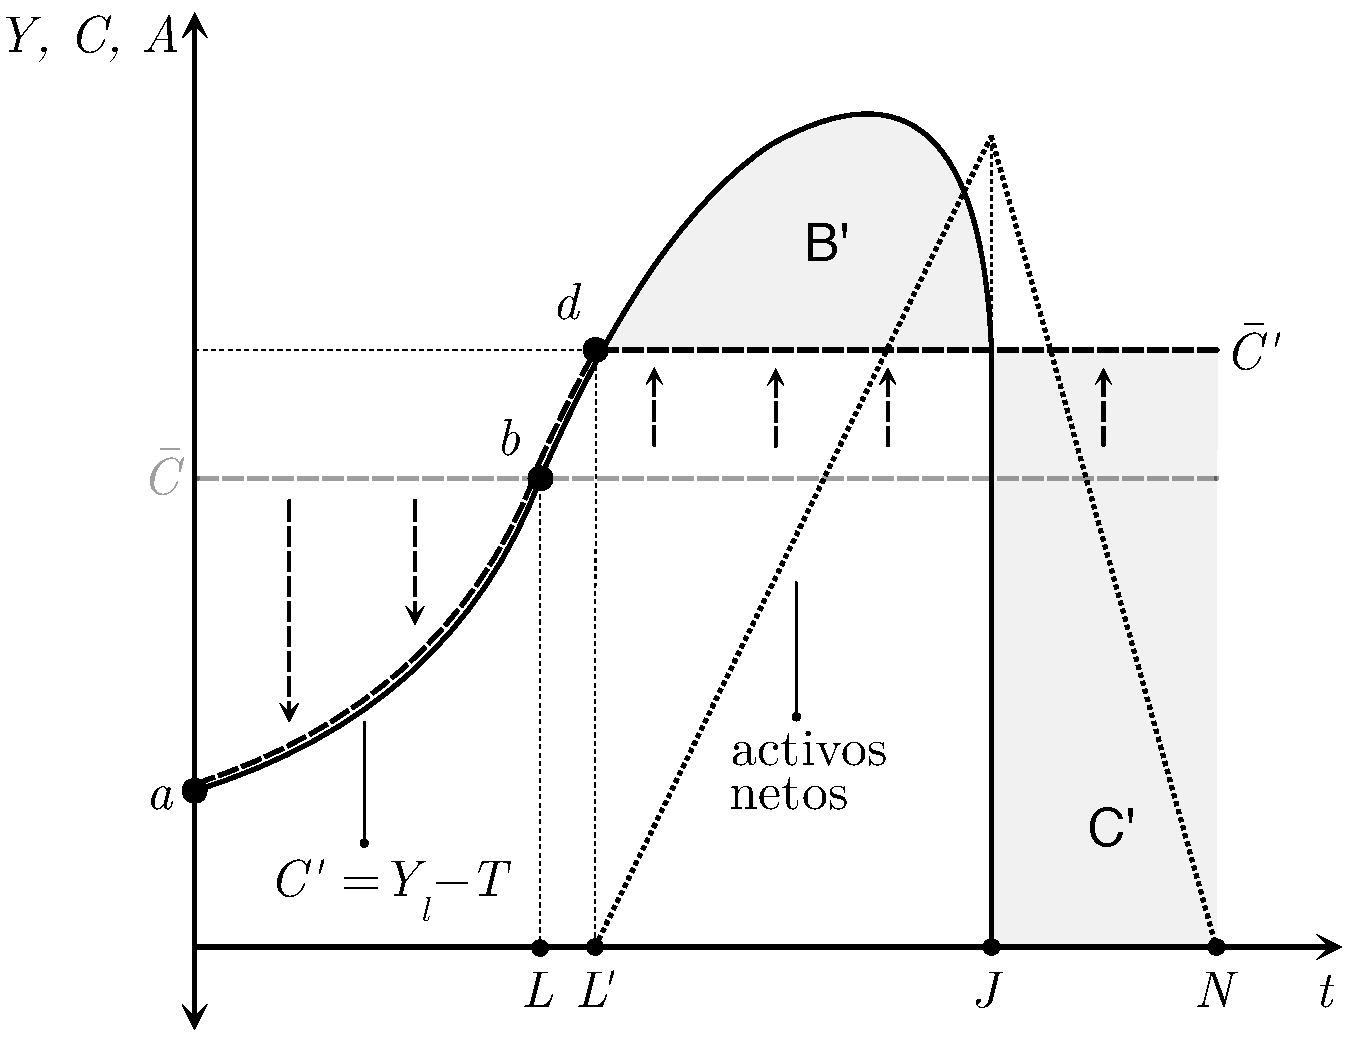
\includegraphics[width=0.5\textwidth]{03_ciclo_vida_rest}
  \caption{Teoría del ciclo de vida con restricción de liquidez}
  \label{fig:ciclo_vida_rest}
\end{figure}

Si hay restricciones de liquidez el consumo en la primera etapa del ciclo de vida está restringido a la trayectoria de ingreso disponible, pero sabemos que el valor de la riqueza total no ha cambiado. Por lo tanto, el consumo promedio con restricción de liquidez será mayor que sin ella ($\bar{C'}>\overline{C}$). Además, dado que no hay deuda, el nivel máximo de activos netos será menor y en general habrá un menor nivel de activos en el mercado de capitales.\footnote{Esto no es lo que sale en el libro, pero se discute en las clases de Alexis Montecinos (Otoño 2011).}

\subsection{Seguridad social}

Una de las principales aplicaciones de la teoría del ciclo de vida es sobre los sistema de pensiones, de los que se pueden distinguir (a grandes rasgos) dos métodos:

\begin{enumdescript}
\item[Sistema de reparto (SR)] (\textit{pay-as-you-go}): quienes trabajan hoy pagan a los jubilados de hoy.
\item[Sistema de capitalización individual (SCI)] (\textit{fully-funded}): quienes trabajan hoy ahorran para su propia jubilación.
\end{enumdescript}

Si las personas ahorran bajo la teoría del ciclo de vida, el SCI no tendría ningún efecto sobre la economía pues todo lo que una persona estuviese obligada a ahorrar lo desahorraría voluntariamente para mantener consumo constante, suponiendo que no hay restricciones de liquidez. Por otro lado, ocurre lo mismo con SR.

Notar que el retorno en SCI corresponde a la tasa de interés de mercado, mientras que el retorno de SR es la tasa de crecimiento de la población y de los ingresos.

¿Por qué existen esquemas de ahorro si la gente podría ahorrar voluntariamente?

\begin{enumdescript}
\item [Inconsistencia intertemporal:] las personas saben que si no ahorran, el gobierno no los dejará pasar pobreza en la vejez y por lo tanto sub-ahorran. Los jóvenes terminan pagando estas pensiones y por eso el estado obliga a aquellos que no ahorraron a hacerlo desde jóvenes.
\item [Mercado del trabajo:] como retirarse del mercado del trabajo es condición necesaria para recibir pensión, se plantea que ésta sería una manera ``más humana'' de retirar a aquellos con baja productividad.
\item [Miopía:] una fracción de la población sería miope y no planifica consumo y ahorro tal como predice la teoría.
\item [Economía política:] los ancianos podrían ser poderosos en el sistema político y presionan por un sistema que redistribuya de los jóvenes a ellos (o vice versa).
\end{enumdescript}

Se argumenta que el SCI tiene una serie de ventajas por sobre SR: libera de influencia de grupos de presión (economía política), sus retornos dependen en menor medida de variaciones demográficas e incentivan la inversión, desarrollando aún más el mercado de capitales.

Sin embargo es relevante ver qué ocurrirá en la práctica cuando se reemplace un SR por un SCI:    los actuales jubilados no tendrán pensión, ya que los jóvenes estarán ahorrando para la de ellos mismos. Entonces será probablemente el fisco quien tendrá que financiar esas pensiones con una deuda pública equivalente al ahorro de los jóvenes.

\subsection{Teoría del ingreso permanente}

Desarrollada por Friedman (1957), propone que el consumidor distingue entre cambios transitorios y permanentes a su ingreso. Los cambios transitorios tendrían efectos pequeños, mientras que los cambios permanentes generarían grandes cambios en los patrones de consumo.

En el modelo de dos períodos es fácil ver este efecto: un cambio en $Y_1$ tendrá un efecto menor que un cambio tanto en $Y_1$ como en $Y_2$. Se puede generalizar esta intuición volviendo a tomar la ecuación \eqref{eq:rest_intertemp_gral} de restricción presupuestaria intertemporal y suponiendo $r=0$, lo que entrega
\begin{equation*}
\sum_{s=0}^{N}{C_{t+s}} = A_t + \sum_{s=0}^{N}{(Y_{l,t+s}-T_{t+i})},
\end{equation*}
donde nuevamente se asume un nivel de consumo constante $\overline{C} \; \forall \: s$, lo que resulta en
\begin{equation}
\overline{C}=\frac{A_t+\sum_{s=0}^{N}{(Y_{l,s}-T_s)}}{N}.
\end{equation}

En general la gente no sabe si el cambio en su ingreso es transitorio o permanente. Una forma sencilla de ligar la teoría del ingreso permanente con la función keynesiana \eqref{eq:consumo_keynesiano} es suponer que las personas consumen una fracción $c$ de su ingreso permanente $Y^p$, es decir,
\begin{equation*}
C_t=c\cdot Y^p_t.
\end{equation*}

Presumiblemente $c$ será cercano a 1. Suponiendo que un ingreso que persiste por dos períodos es permanente y solo una fracción $\theta$ del ingreso corriente es permanente, se define
\begin{align*}
Y^p_t &= \theta Y_t+(1-\theta)Y_{t-1} \\
\implies C_t &= c\cdot \theta Y_t+c\cdot(1-\theta)Y_{t-1}.
\end{align*}

Entonces,

\begin{align*}
PMgC^{CP} &= c\cdot\theta \\
PMgC^{LP} &= c.
\end{align*}

Sofisticando un poco más la teoría del ingreso permanente, se supone un individuo que no tiene activos hasta el tiempo $t$, tiene horizonte infinito e ingreso constante $Y$. Ahora, si repentinamente recibe un ingreso $\overline{Y}>Y$ y cree que se mantendrá así con probabilidad $p$, entonces se puede denotar el valor presente de sus ingresos en caso de que el cambio sea permanente como $V_a$, mientras que el valor presente de un cambio transitorio será $V_b$, de forma que

\begin{align*}
V_a &= \frac{1+r}{r}\overline{Y} \\
V_b &= \overline{Y}+\frac{Y}{r}.
\end{align*}

Luego, usando la ecuación de consumo recién definida pero reemplazando $\theta=p$, $Y_t=V_a$ y $Y_{t-1}=V_b$ ($c=1$) y tomando su valor presente, se tiene que
\begin{align*}
C_t &= \frac{r}{1+r}[pV_a+(1-p)V_b] \\
%&= \frac{r}{1+r}\left[p\frac{1+r}{r}\overline{Y}+(1-p)\overline{Y}+(1-p)\frac{Y}{r}\right] \\
%&= p\overline{Y}+\frac{r}{1+r}(1-p)\overline{Y}+\frac{Y(1+r)(1-p)}{r} \\
%&= p\overline{Y}+\frac{r}{1+r}(1-p)\overline{Y} + \frac{Y(1-p+r-rp)}{r} \\
C_t &= \frac{p+r}{1+r}\overline{Y}+\frac{1-p}{1+r}Y.
\end{align*}

Ahora se puede definir la propensión marginal a consumir como la razón del cambio en consumo sobre el cambio en ingreso, $	\Delta C/\Delta Y$. Usando la expresión recién calculada para $C_t$ y usando el hecho de que $C_{t-1}=Y$ (porque en $t-1$ no había habido shock de ingreso) es fácil calcular que
\begin{equation}
PMgC \approx \frac{C_t-C_{t-1}}{\overline{Y}-Y} = \frac{p+r}{1+r},
\end{equation}
donde $PMgC$ es creciente en $p$ y, además, es igual a 1 cuando $p=1$.

Un análisis interesante que es propuesto es ver qué ocurriría si la alternativa a $\overline{Y}$ fuese un ingreso $\breve{Y}$ aún mayor, es decir, $\breve{Y}>\overline{Y}$. En este caso, se observará que
\begin{equation*}
C'_t=\frac{p+r}{1+r}\overline{Y}+\frac{1-p}{1+r}\breve{Y}.
\end{equation*}
de donde se desprende que $C'_{t}>C_{t} \quad \forall \; p<1$. Dado que  $C_{t-1}$ no cambia, es lógico decir que $C_t-C_{t-1}<C'_t-C_{t-1}$. Además se tiene que el cambio en ingreso $\overline{Y}-Y$ sigue siendo el mismo, por lo que se puede asegurar que la nueva propensión marginal a consumir es superior a la del caso anterior. Esto porque cambió el consumo presente en mayor proporción que el ingreso.

Mas interesante aún es demostrar no solo que la nueva $PMgC'$ es mayor a la anterior, si no además que es mayor que 1. Yo lo hice de la siguiente forma:

\begin{align*}
C'_t-C_{t-1} &= \left[\frac{p+r}{1+r}\overline{Y}-Y\right]+\frac{1-p}{1+r}\breve{Y} \\
 &= \left[C_t-C_{t-1}-\frac{1-p}{1+r}\overline{Y}\right]+\frac{1-p}{1+r}\breve{Y} \quad \bigg|\cdot \frac{1}{\overline{Y}-Y} \\
PMgC'=\frac{C'_t-C_{t-1}}{\overline{Y}-Y}&= \frac{p+r}{1+r} + \frac{1-p}{1+r}\cdot\frac{\breve{Y}-Y}{\overline{Y}-Y}.
\end{align*}

Esta es la expresión a probar que sea mayor que 1 ($PMgC'>1$), es decir,
\begin{equation*}
\frac{p+r}{1+r} + \frac{1-p}{1+r}\cdot\frac{\breve{Y}-Y}{\overline{Y}-Y} > 1.
\end{equation*}

Después de un poco de álgebra se llega a que la condición para que dicha expresión se cumpla es $\breve{Y}>\overline{Y}$, lo cual corresponde al supuesto inicial.

Ambas teorías predicen que el efecto de un cambio en el ingreso sobre el consumo es proporcional al incremento en la riqueza total producto del incremento en el ingreso (sea transitorio o permanente). Suponen un agente de horizonte infinito y completa certidumbre sobre el futuro, sin restricciones de liquidez.

\subsection{Consumo, incertidumbre y precios de activos}

\subsubsection{Implicaciones estocásticas de la teoría del consumo}

Se supone un individuo que resuelve
\begin{equation*}
\max_{C_t,C_{t+1}} u(C_t)+\frac{1}{1+\rho}\E_{t}[u(C_{t+1})] \sa Y_t+\frac{Y_{t+1}}{1+r}=C_t+\frac{C_{t+1}}{1+r},
\end{equation*}
donde $\rho $ es la tasa de descuento y $r$ es una tasa de interés libre de riesgo. Despejando la restricción para $C_{t+1}$ y reemplazando en la función de utilidad, la condición de primer orden del problema es
\begin{equation*}
u'(C_t)= \frac{1+r}{1+\rho} \E_{t}[u'(C_{t+1})].
\end{equation*}

Al suponer $r=\rho$ y una función de utilidad cuadrática de la forma $u(C)=-(\overline{C}-C)^2$ se llega a
\begin{equation*}
C_t=\E_t[C_{t+1}],
\end{equation*}
es decir, el valor esperado del consumo en $t+1 $ es igual al consumo de $t $. Esto es así porque el valor esperado toma en cuenta toda la información disponible en $t$ y el único origen de desviación en el patrón de consumo serán shocks inesperados al consumo:
\begin{equation}
\sscript{C}{t+1}=\sscript{C}{t}+\sscript{\xi}{t+1},
\end{equation}
donde $\xi$ es un shock inesperado al consumo con $\E_{t}[\sscript{\xi}{t+1}]=0$.

De aquí se deriva el resultado de Hall (1978), en donde demostró que bajo las condiciones recién descritas la teoría del CV/IP implica que el consumo sigue un \textit{random walk} o camino aleatorio. Notar que todos los shocks al consumo son permanentes en este caso particular. De hecho si $\sscript{C}{t+1}=\delta C+\xi_{t+1}$ con  $\delta=1$, es decir, un camino aleatorio, un shock unitario al consumo elevará este shock en 1 permanentemente.\footnote{Si $\delta<1$ entonces es un proceso autoregresivo de orden 1 y por lo tanto el efecto del shock será transitorio, ya que los consumos futuros ($C_t$ con $t>1$) serán ponderados por $\delta^{t-2}$.} Este resultado es generalizable más allá de las funciones de consumo cuadráticas. Sin embargo, la evidencia empírica sugiere que el consumo no sigue un camino aleatorio.

\subsubsection{Precios de activos, el modelo CAPM y el puzzle de premio de las acciones}

Si el individuo tiene acceso a comprar un activo $i$ con retorno incierto igual a $r^i$, en cuyo caso la CPO del problema sería
\begin{equation*}
u'(C_t)= \E_t \left[\frac{1+r^i}{1+\rho} u'(C_{t+1}) \right].
\end{equation*}

Luego se define al \textbf{factor de descuento estocástico} $M$ como
\begin{equation}
M= \frac{u'(C_{t+1})}{(1+\rho)u'(C_t)}
\end{equation}
y por lo tanto la CPO puede expresarse como
\begin{equation*}
\E_t[(1+r^i)\cdot M] = \E_t[M] + \E_t[r^i\cdot M]=1.
\end{equation*}

Usando que $\text{Cov}(X,Y)=\E[XY]-\E[X]\cdot \E[Y] $, la expresión anterior es
\begin{equation*}
\E_t[M]+\E_t[r^i\cdot M] = \E_t[M] + \E_t[r^i]\E_t[M]+ \text{Cov}(r^i, M) = 1.
\end{equation*}

Si esta condición se cumple para el activo libre de riesgo, se tiene que
\begin{equation*}
(1+r)\E_t[M] = E_t[M]+r\E_t[M]=1.
\end{equation*}

Combinando las últimas dos ecuaciones y recordando que $1+\rho$ y $u'(C_t)$ no son estocásticos, se llega a que una expresión para el \textbf{exceso de retorno} es
\begin{equation}
\E_t[r^i]-r = -\frac{\text{Cov}(r^i,M)}{\E_t[M]} = -\frac{\text{Cov}(r^i,u'(C_{t+1}))}{\E_t[u'(C_{t+1})]}.
\label{eq:exceso_retorno}
\end{equation}

Esta expresión muestra el premio de un activo riesgoso por sobre uno libre de riesgo. Asumiendo que la covarianza del retorno y la utilidad marginal del consumo son negativas, entonces la prima del activo será positiva. De esto se concluye que cuando el retorno de un activo covaría positivamente con el consumo, requerirá pagar un premio positivo.

Ahora se puede econtrar cuánto debería ser el precio de un activo cualquiera respecto de la tasa libre de riesgo, cuya relación en finanzas es el \textbf{modelo CAPM}. Se supone un activo cuyo retorno $r^m$ está perfecta y negativamente correlacionado con la utilidad marginal del consumo, es decir,
\[
r^m = -\theta u' (C_{t+1}).
\]

La covarianza entre $r^m$ y $(C_{t+1})$ será $-\text{Var}(r^m)/\theta$, es decir, el activo tendrá un exceso de retorno positivo con respecto de la tasa libre de riesgo. Análogamente, la covarianza de un activo cualquiera $i$ con retorno $r^i$ y $u'(C_{t+1})$ será igual a $-\text{Cov}(r^i, r^m)/\theta$. Usando esto para ambos activos en la ecuación \eqref{eq:exceso_retorno} significa que
\begin{align*}
\E_t[r^i]-r &= \frac{\text{Cov}(r^i, r^m)}{\theta \E_t u'(C_{t+1})} \\
\E_t[r^m]-r &= \frac{\text{Var}(r^m)}{\theta \E_t u'(C_{t+1})}.
\end{align*}

Ahora, usando ambas ecuaciones para eliminar $E_t u'(C_{t+1)}$ se llega a
\begin{equation}
E_t r^i - r = \beta^i(E_tr^m - r),
\label{eq:CAPM}
\end{equation}
donde $\beta^i = \frac{\text{Cov}(r^i, r^m)}{\text{Var}(r^m)} $. La ecuación \eqref{eq:CAPM} corresponde a la ecuación de precios de activos del CAPM.

\begin{itemize}
\item Si $\beta>1$ el activo covaría positivamente con el mercado y es más volátil ($\text{Cov}(r^i, r^m)>\text{Var}(r^m)$) su retorno debería ser mayor al del mercado, pues requiere un premio para que el público lo mantenga.
\item Si $0<\beta<1$ el activo covaría positivamente con el mercado pero su retorno es estable ($\text{Cov}(r^i, r^m)<\text{Var}(r^m)$) entonces el retorno será menor que el de mercado pero mayor que el libre de riesgo, pues este activo es más seguro que el mercado y requiere menor prima por riesgo.
\item Si $\beta<0$ el activo covaría negativamente con el mercado y su retorno será menor que el libre de riesgo, ya que sirve adicionalmente como seguro para cubrirse de riesgos. $\blacksquare$
\end{itemize}

% Quizás incluir discusión final con distintas especificaciones de U que concilian a la teoría con la evidencia empírica. Incluir equity premium puzzle.

\end{document}